\chapter{Simulation study}
\label{chap:SimulationStudy}

\section{Introduction}
In order to study the methods in more depth a simulation study will be done. The main advantage of this simulation study over using data on real species is that the variables that make up the species distribution can be decided upon. Because of the usual non-linear shape of the response-functions, the sampling design, \dots it is quite hard to set up a simulation study. Luckily the
\textsc{virtualspecies} package \parencite{virtualspecies, leroy2015virtualspecies} provides a simulation framework that allows the simulation of realistic species distributions. \\

\section{Overview of the \textsc{virtualspecies} package and the simulation set-up}
In order to justify using the samples generated by the \textsc{virtualspecies} package the internal process is quickly sketched. \\

First of all, the \textsc{virtualspecies} package generates a suitability raster, i.e.\ a raster containing high values for suitable habitat and vice versa, based upon a set of provided rasters of environmental variables. Since the package imposes no restrictions on the function that generates the values associated with the presence locations suitability from the provided variables, the suitability raster has to be converted into a probability of occurrence map. This can be done by using e.g.\ the logit function to map $\mathbb{R} \to [0,1]$. Once a raster containing the occurrence probability map is obtained a raster containing ones where the simulated species is present and zeroes otherwise can be obtained. This is done by sampling cells with a probability proportional to the probability of the occurrence and setting the cell value to $1$. From this raster a presence-only sample can be obtained by drawing random points within the cells that have a value of $1$.\\

It is interesting to note that the suitability raster is based upon the principal components of the variables over the whole study extent. Hence in our simulation study it is in some sense more appropriate to perform the (K)PCA logistic regression on the background points. \\

To facilitate the computations it was decided to select one area in which several random species are generated. In order to make sure that the environmental conditions can fluctuate within the distribution of one generated species to the next it was required that the selected area has to contain different types of habitat types. The obvious choice would be to use the contiguous United States, this is, however, computationally demanding. In the end it was decided to perform the simulation study on data contained within a rectangle that approximately corresponds to Washington state, see Figure \ref{fig:WashState}. Washington state has a big precipitation and temperature gradient because of the rain shadow created by the Cascade Range. This is also reflected in the fact that the types of habitat within this extent range from temperate rainforests, e.g.\ the Hoh Rainforest, to steppe- and dessert-like areas in Southeastern Washington.

\begin{figure}[!htb]
\center
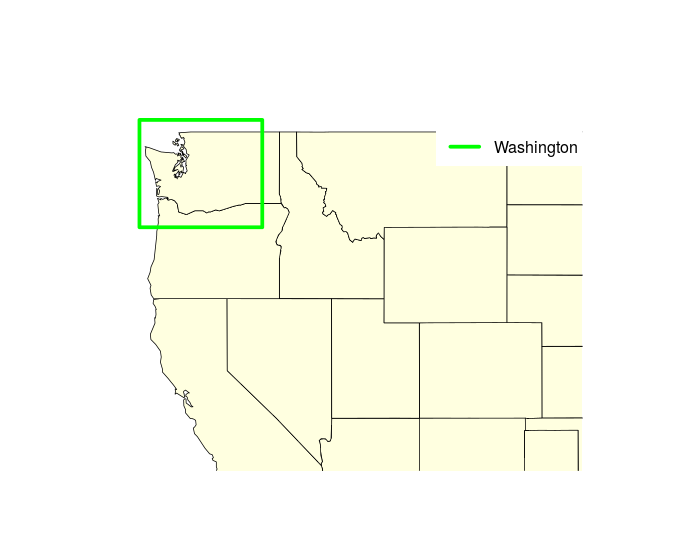
\includegraphics[scale=0.5]{Plots/WashingtonPlot.png}
\caption{\label{fig:WashState}Extent considered in the simulation study.}
\end{figure}

In order to study the generalizability of the methods it was decided that $5$ different species would be simulated. Furthermore, to be able to investigate the sample to sample variability of each method $5$ different presence-only samples were drawn for each simulated species. Since the mean (resp.\ median) number of observations of the presence-only datasets is $320.3$ (resp.\ $133.5$) it was decided to simulate $200$ occurrence points for each simulated dataset. \\

In Section \ref{sec:AUC} the various sources of the variability in the AUC values were discussed. Given that the interest is mainly in the training sample to training sample variability, it was decided to try to restrict the test sample to test sample variability to some extent. This can be done by taking a large test set. Using a sample of $1000$ occurrence and $1000$ background locations the standard error of the AUC value, conditional on the classifier, is $\approx 0.013$. This should be large enough to prevent the scenario where the test sample to test sample variability is much larger than the training to training sample variability.

\section{Model and estimators}
\label{sec:Estimators}
In order to be able to perform statistical inference an underlying model has to be proposed and estimators will be proposed. First of all the generated AUC values will be denoted by $Y_{ij}$ with $i \in \{1,\ldots,5\}$ indicating the species and $j \in \{1,\ldots,5\}$ indicates which sample of the $i$'th virtual species is considered. We assume that there is an underlying average AUC value $\mu$, for each sampled species there is then a species specific average AUC that deviates from $\mu$ by an amount equal to $\delta_i$ with $E(\delta_i) = 0$. Finally, because of training and test sample variability the estimated AUC will deviate from $\mu + \delta_i$ by an error $\epsilon_{ij}$ with $E(\epsilon_{ij}) = 0$. Hence:

\begin{equation}
\label{eq:SimModel}
Y_{ij} = \mu + \delta_i + \epsilon_{ij}.
\end{equation}

It is logically to assume that not only the $\delta_i$ and $\epsilon_{ij}$ are random but also that the $\text{Var}(\epsilon_ij) = \sigma_i^2$ is a species specific variance that is different for each species. For each method we are interested is in estimating:
\begin{itemize}
\item The mean $\mu$.
\item The expected variation of a classifier ``independent'' of the selected species or hence $E(\sigma^2) \equiv \tau^2$.
\item The difference between using all variables or only the bioclimatic variables, i.e. $\mu_{all} - \mu_{bio}$.
\end{itemize} 
It could be argued that also the species to species variance is of interest, however since we're considering virtual species generated by a specific process this would probably not represent the real world species to species variability. \\

First of all the usual unbiased estimator of $\sigma_i^2$ is $\sum_{j= 1}^{5} \frac{(Y_{ij} - \bar{Y}_i)^2}{4} $, with $\bar{Y}_i = \frac{\sum_{j=1}^{5}Y_{ij}}{5}$.
In order to estimate $\tau^2$ we note that 

\begin{align*}
E\left(\frac{1}{5} \sum_{j= 1}^{5} \frac{(Y_{ij} - \bar{Y}_i)^2}{4}\right)
 & = E\left\lbrace \frac{1}{5} \sum_{i=1}^5 E\left( \sum_{j= 1}^{5} \frac{(Y_{ij} - \bar{Y}_i)^2}{4}  \bigg\vert \sigma_1^2, \ldots, \sigma_5^2 \right) \right\rbrace \\
& = \frac{1}{5} \sum_{i=1}^5 E \left( \sigma_i ^ 2 \right)  \\
& = E\left( \sigma^2 \right). 
\end{align*}
Hence
 \[\hat{\tau}^2 = \frac{1}{5} \sum_{j= 1}^{5} \frac{(Y_{ij} - \bar{Y}_i)^2}{4}\]
 is an unbiased estimator of $\tau^2$. It seems reasonable to use 
\[ 
 \hat{\tau} =\sqrt{\frac{1}{5} \sum_{j= 1}^{5} \frac{(Y_{ij} - \bar{Y}_i)^2}{4}} \]
as a biased estimator of $\tau$. In order to say obtain confidence intervals (CI) of $\hat{\tau}$ bootstrapping will be used. Intuitively one would expect that the following two-stage scheme is the most appropriate:
\begin{enumerate}
\item Sample $5$ species with replacement.
\item Sample $5$ of the observations with replacement for each sampled species.
\item Calculate $\hat{\tau}$ for each bootstrap sample.
\end{enumerate}
However, in \cite{field_bootstrapping_2007} it was theoretically deduced that it is better to not perform the second step in this bootstrap algorithm and hence only the species are sampled with replacement. This was also shown with simulation studies performed in \cite{ren_nonparametric_2010}. Hence, we will only resample the species. Since the results in \cite{field_bootstrapping_2007} are based on a setting which is closely related to ours and they showed that the variance of the within sum of squares is underestimated and underestimation of the variance of $\hat{\tau}$ is to be expected. \\
  
In order to estimate $\mu$ for each method and for the models using all or only the bioclimatic variables generalized ordinary least squares will be used. GLS was opted for instead of ordinary least squares because it allows for unequal variances within species. Although the residual distribution cannot be normal, the AUC is bounded up- and downwards, we will assume they are approximately normally distributed. To check how reasonable this is QQ-plots of the residuals will be constructed. Finally, perhaps all the inference could be done by fitting one large mixed model including effects for the method used, etc. However trying to do so complicates the model estimation and allowing for enough flexibility, e.g.\ having a realistic correlation structure, for such a model to be realistic is hard and leads to identifiability issues. 

\section{Results}
Before discussing the results we refer to the QQ-plots in Figure \ref{fig:ResidualGLSAll}, \ref{fig:ResidualGLSBio}, and \ref{fig:ResidualGLSDiff} in the Appendix \ref{ch:plots}. The QQ-plots seem to indicate that the residuals seem to have slightly light tails. This could be expected since the AUC values are bounded up and downwards. However, it seems quite reasonable to assume that this slight deviation does not cause any real problems when inference is performed. Hence, it seems like our GLS models are a good fit. A plot of the AUC values can be found in Figure \ref{fig:AUCSimulation} and a plot of the difference between the AUC using all minus only the bioclimatic variables can be found in Figure \ref{fig:DiffSimulation}. The estimated means and their SEs can be found in Table \ref{tab:AUCSimulation}. The estimated SDs and $95$\% CIs based on $100000$ bootstrap samples can be found in Table \ref{tab:SDSimulation}. Histograms of the bootstrap samples can be found in Figure \ref{fig:BootstapAll}, \ref{fig:BootstapBio}, and \ref{fig:BootstapDiff} in Appendix \ref{ch:plots}\\

\begin{table}[!htb]
\makebox[\textwidth][c]{
\begin{tabular}{lcccccc}
 & \multicolumn{2}{c}{All variables} & \multicolumn{2}{c}{Bioclimatic variables} & \multicolumn{2}{c}{Difference}\\
\cline{2-3} \cline{4-5} \cline{6-7}\\
Method & Mean AUC & SE & Mean AUC & SE & Mean AUC & SE \\
\midrule
Logistic: vanilla                 & 0.784 &   0.016 & 0.794 & 0.003 & 0.010     & 0.017\\ 
Logistic: backward                & 0.533 &   0.026 & 0.607 & 0.027 & 0.074     & 0.041\\
Logistic: forward                 & 0.489 &   0.029 & 0.546 & 0.019 & 0.057     & 0.037\\
Logistic: PCA                     & 0.790 &   0.004 & 0.789 & 0.004 & -0.001    & 0.005\\
Logistic: presence PCA            & 0.797 &   0.005 & 0.774 & 0.010 & -0.023    & 0.011\\
Logistic: background PCA          & 0.794 &   0.003 & 0.787 & 0.004 & -0.008    & 0.005\\ 
Logistic: kernel PCA              & 0.807 &   0.002 & 0.807 & 0.005 & 0.000     & 0.004\\ 
Logistic: presence kernel PCA     & 0.810 &   0.003 & 0.810 & 0.004 & 0.000     & 0.004\\ 
Logistic: background kernel PCA   & 0.807 &   0.003 & 0.810 & 0.004 & 0.003     & 0.004\\ 
Logistic: lasso                   & 0.806 &   0.003 & 0.806 & 0.004 & 0.000     & 0.004\\ 
Logistic: ridge                   & 0.800 &   0.003 & 0.798 & 0.003 & -0.002    & 0.004\\ 
Logistic: select07                & 0.754 &   0.014 & 0.787 & 0.018 & 0.033     & 0.025\\ 
GAM: auto selection               & 0.809 &   0.002 & 0.807 & 0.004 & -0.003    & 0.004\\ 
GAM: vanilla                      & 0.805 &   0.002 & 0.809 & 0.004 & 0.004     & 0.004\\ 
GAM: select07                     & 0.804 &   0.002 & 0.804 & 0.004 & -0.001    & 0.005\\ 
MaxEnt                            & 0.772 &   0.005 & 0.766 & 0.008 & -0.006    & 0.007\\
MaxEnt Vanilla                    & 0.702 &   0.012 & 0.728 & 0.012 & 0.026     & 0.014\\
ANN                               & 0.801 &   0.003 & 0.814 & 0.005 & 0.012     & 0.006\\
ANN: vanilla                      & 0.793 &   0.003 & 0.797 & 0.006 & 0.004     & 0.007\\
GBM                               & 0.811 &   0.002 & 0.809 & 0.006 & -0.002    & 0.006\\
\bottomrule
\end{tabular}}
\caption{\label{tab:AUCSimulation}Summary of the AUC values of the different classifiers fitted on the simulated data.}
\end{table}

\begin{figure}[!htb]
\center
\makebox[\textwidth][c]{%
	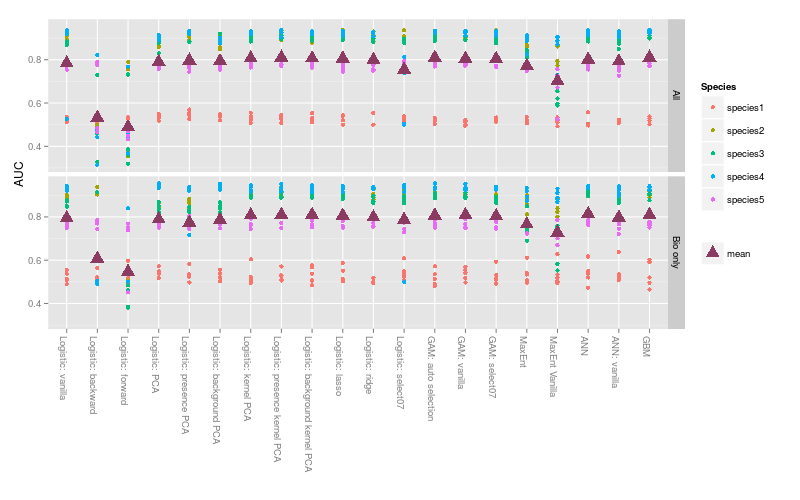
\includegraphics[scale=0.70]{Plots/SimulationAUC.png}
}
\caption{\label{fig:AUCSimulation}AUC values of the different classifiers fitted on the simulated data.}
\end{figure}


\begin{figure}[!htb]
\center
\makebox[\textwidth][c]{%
	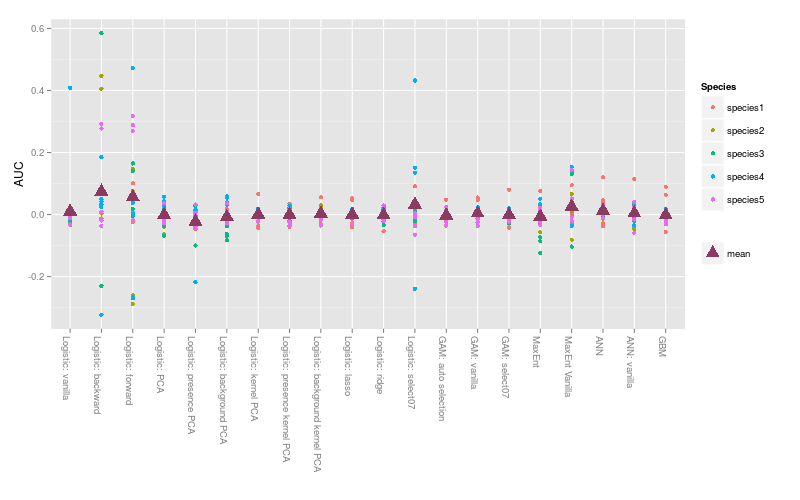
\includegraphics[scale=0.70]{Plots/SimulationDifference.png}
}
\caption{\label{fig:DiffSimulation}Difference between the AUC values when using all versus only the bioclimatic variables.}
\end{figure}

The mean AUCs largely confirm the conclusions made in Chapter \ref{ch:Applications}. In particular logistic regression performs quite well on its own. Techniques that allow for flexible non-linear relations tend to have the highest mean AUC. It is particularly interesting that MaxEnt, especially when the default parameters are used, performs quite badly. The penalized regression models seem approximately on par with the logistic regression model. The select07 logistic regression methods seems perform slightly worse than standard logistic regression. \\ 

When it comes to the stepwise methods the results diverge slightly from what was observed in Chapter \ref{ch:Applications}. More particularly the stepwise methods perform even worse. When all variables are considered these methods have a mean AUC around $0.5$ which is the same as one would get when a classifier that randomly labels the observations as presences or background points. \\

It is striking that there is no noticeable difference between performing (K)PCA on the predictor values corresponding to all, the presence, or the background locations. Given the way the virtual species were generated it was expected that the (K)PCA performed on the predictor values corresponding to background points would be superior. Hence, based on the mean AUC there seems to be no reason to prefer one over the other. \\

None of the methods perform significantly worse when the non-relevant, i.e.\ non-bioclimatic, variables are added. However, it seems reasonable that some models perform somewhat worse: especially logistic regression model, MaxEnt with the default parameters, and the stepwise models show quite a decrease. If a more extensive simulation study would be performed extra interest could be in these methods. \\

\begin{table}[!htb]
\makebox[\textwidth][c]{
\begin{tabular}{lcccccc}
 & \multicolumn{2}{c}{All} & \multicolumn{2}{c}{Bioclimatic} & \multicolumn{2}{c}{Difference} \\
 \cline{2-3} \cline{4-5} \cline{6-7}\\
 Method & $\hat{\tau}_{all}$ & 95\% CI  &  $\hat{\tau}_{bio}$ & 95\% CI &  $\hat{\tau}_{bio} - \hat{\tau}_{all}$ & 95\% CI \\

\midrule
Logistic: vanilla                 & 0.081 &  [0.009; 0.140] & 0.015  & [0.009; 0.022] & -0.066 &  [-0.130; 0.012]   \\ 
Logistic: backward                & 0.131 &  [0.067; 0.173] & 0.134  & [0.017; 0.198] & 0.003  &  [-0.143; 0.104]   \\
Logistic: forward                 & 0.143 &  [0.071; 0.190] & 0.096  & [0.037; 0.133] & -0.047 &  [-0.137; 0.041]   \\
Logistic: PCA                     & 0.021 &  [0.012; 0.030] & 0.018  & [0.013; 0.022] & -0.003 &  [-0.011; 0.007]   \\
Logistic: presence PCA            & 0.024 &  [0.012; 0.034] & 0.048  & [0.021; 0.076] & 0.024  &  [-0.008; 0.061]   \\
Logistic: background PCA          & 0.017 &  [0.012; 0.023] & 0.018  & [0.014; 0.021] & 0.001  &  [-0.008; 0.007]   \\ 
Logistic: kernel PCA              & 0.012 &  [0.008; 0.015] & 0.024  & [0.013; 0.035] & 0.012  &  [0.004; 0.020]   \\ 
Logistic: presence kernel PCA     & 0.014 &  [0.010; 0.017] & 0.018  & [0.014; 0.022] & 0.005  &  [0.000; 0.009]   \\ 
Logistic: background kernel PCA   & 0.013 &  [0.009; 0.017] & 0.022  & [0.013; 0.032] & 0.009  &  [0.001; 0.017]   \\ 
Logistic: lasso                   & 0.014 &  [0.010; 0.018] & 0.021  & [0.011; 0.030] & 0.006  &  [0.000; 0.013]   \\ 
Logistic: ridge                   & 0.016 &  [0.011; 0.021] & 0.015  & [0.010; 0.019] & -0.001 &  [-0.008; 0.004]   \\ 
Logistic: select07                & 0.068 &  [0.008; 0.117] & 0.090  & [0.018; 0.152] & 0.022  &  [0.004; 0.035]   \\ 
GAM: auto selection               & 0.011 &  [0.008; 0.013] & 0.020  & [0.011; 0.030] & 0.009  &  [0.000; 0.019]   \\ 
GAM: vanilla                      & 0.010 &  [0.008; 0.012] & 0.018  & [0.011; 0.025] & 0.008  &  [0.000; 0.014]   \\ 
GAM: select07                     & 0.011 &  [0.008; 0.013] & 0.021  & [0.011; 0.031] & 0.010  &  [0.000; 0.022]   \\ 
MaxEnt                            & 0.023 &  [0.016; 0.030] & 0.039  & [0.025; 0.050] & 0.015  &  [-0.001; 0.029]   \\
MaxEnt Vanilla                    & 0.062 &  [0.038; 0.081] & 0.062  & [0.039; 0.083] & 0.000  &  [-0.036; 0.036]   \\
ANN                               & 0.016 &  [0.010; 0.022] & 0.025  & [0.008; 0.041] & 0.009  &  [-0.002; 0.020]   \\
ANN: vanilla                      & 0.016 &  [0.011; 0.020] & 0.029  & [0.015; 0.043] & 0.013  &  [-0.003; 0.031]   \\
GBM                               & 0.012 &  [0.008; 0.015] & 0.029  & [0.010; 0.047] & 0.017  &  [-0.002; 0.035]   \\
\bottomrule
\end{tabular}}
\caption{\label{tab:SDSimulation}Estimates and bootstrapped confidence intervals of the standard deviation $\tau$.}
\end{table}

An inspection of Table \ref{tab:SDSimulation} indicates roughly that $\tau$ shows roughly the same trends as those observed in Chapter \ref{ch:Applications}. First of all the logistic regression model is quite stable when only the bioclimatic variables are considered. Once extra redundant variables are added there is a large increase in the SD. However, $0$ is included in the $95$\% CI so rigorously we cannot conclude that the SD increases. The other methods seem quite stable, which since variable selection techniques are added is to some extent what is expected. Note that $8$ of the $95$\% CI only include positive values, this would lead to the conclusion that including irrelevant variables improves the classifiers. Of course this is non-sensical and this behaviour can likely be related to the underestimation of the variance in the bootstrap procedure, see Section \ref{sec:Estimators}. \\

Just as for the mean AUC the methods that allow for flexible non-linear relations tend 
to perform the best, i.e.\ have the lowest $\hat{\tau}$ vales. Furthermore, the MaxEnt implementation that uses the default parameters has quite a high $\hat{\tau}$ and also its $95$\% CI includes relatively high values. The penalized regression methods perform quite well. In particular when the only the bioclimatic variables are considered their SD is on par with the SD of logistic regression. When all the variables are considered the SD, unlike what was the case for logistic regression, stays stable. The no influential trend is seen when the (K)PCA is performed on the different observations. Hence again there seems to be no effect of the presence vs background location. Finally, both stepwise methods are the worst methods, i.e.\ most variable, of the methods considered. The select07 method combined with logistic regression seems quite variable, this is not completely in line with the results of Section \ref{sec:POData}.


\section{Conclusion}




